\chapter{The SuperNEMO demonstrator}
\label{ch:detector}

\section{Demonstrator design}
\subsection{Comparison with NEMO$3$ experiment}
\subsection{Expermimental design}
\subsection{Sources}
\begin{itemize}
\item Choice of source material
\end{itemize}

\subsection{Tracker}
\subsection{Calorimeter}
\label{subsec:SN_calo}



\subsubsection{Scintillator}





\subsubsection{Photomultiplier}
\label{sec:calorimeter}
\subsection{Calibration systems}
\subsection{Control Monitoring system}
\subsection{Electronics}

\section{The backgroung of SuperNEMO}
\label{sec:SNbkg}
\subsection{Internal background}
\label{subsec:SNbkg_internal}

Trace quantities of naturally-occurring radioactive isotopes can occasionally produce two-electron events and thus can mimic $\beta\beta$-decay events.
The largest contributions come from isotopes of decay chains of $^{238}$U, $^{232}$Th and $^{40}$K, which disintegration occur inside the source foils, as well as inside the tracking volume.

Décire la contamination mesurée des sources, et du radon dans la partie suivante

\begin{figure}[!h]
\centering
\begin{subfigure}[t]{0.32\textwidth}
  \centering
  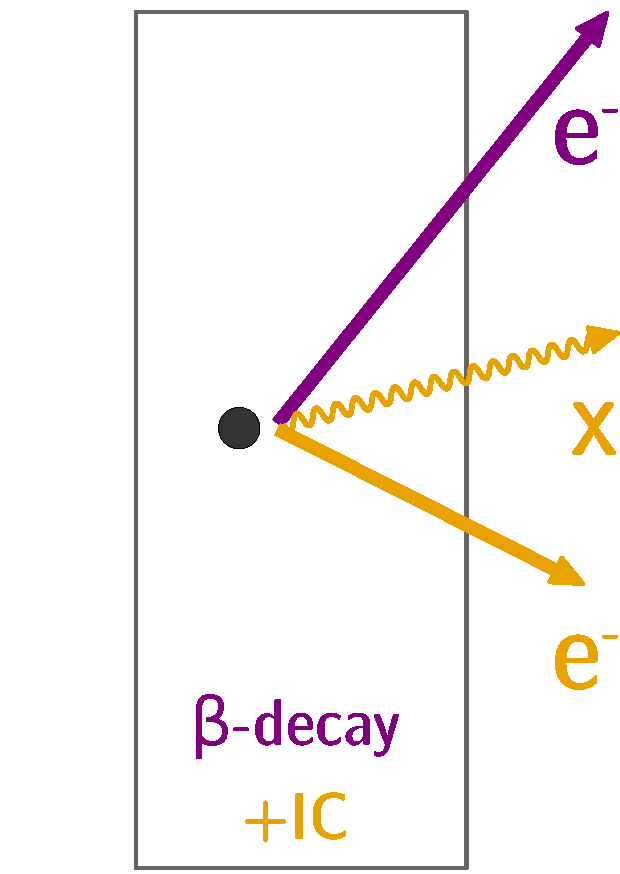
\includegraphics[width=0.82\textwidth]{SNdemonstrator/fig_SNdemonstrator/internal_contamination_IC.pdf}
  \captionsetup{justification=justified}
  \caption{
    \label{subfig:cont_Pint_eff}}
\end{subfigure}
\hfill
\begin{subfigure}[t]{0.32\textwidth}
  \centering
  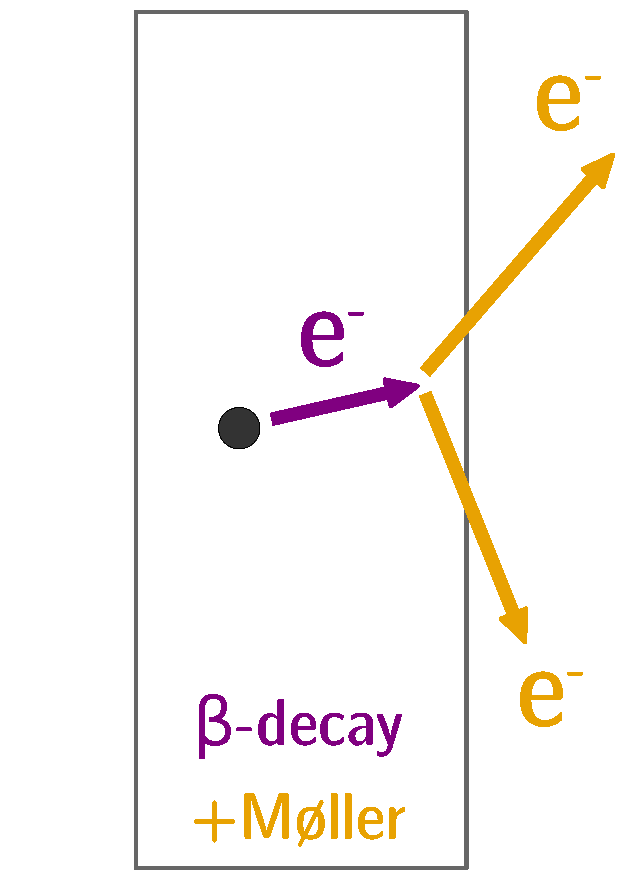
\includegraphics[width=0.82\textwidth]{SNdemonstrator/fig_SNdemonstrator/internal_contamination_moller.pdf}
  \captionsetup{justification=justified}
  \caption{
    \label{subfig:cont_Pint_ROI}}
\end{subfigure}
\hfill
\begin{subfigure}[t]{0.32\textwidth}
  \centering
  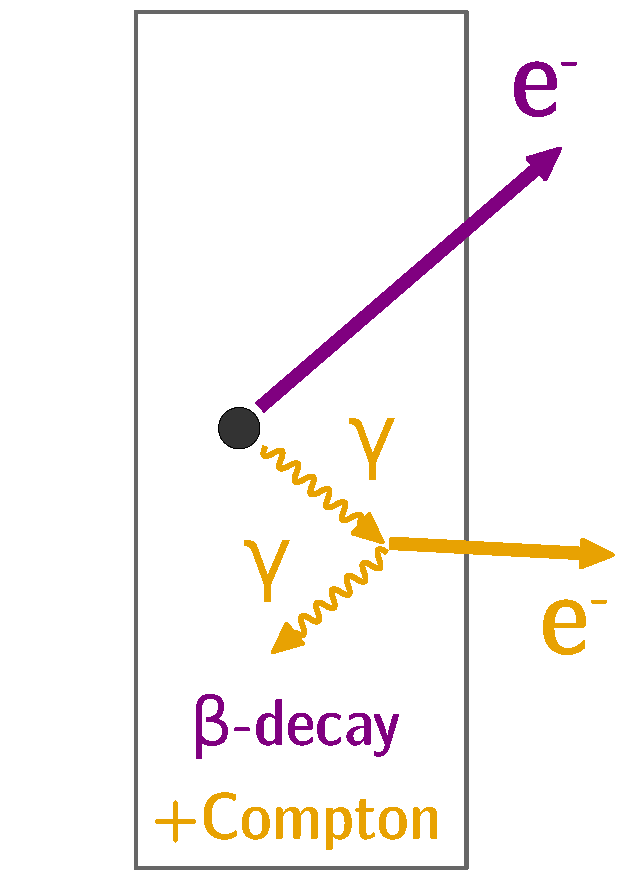
\includegraphics[width=0.82\textwidth]{SNdemonstrator/fig_SNdemonstrator/internal_contamination_compton.pdf}
  \captionsetup{justification=justified}
  \caption{
    \label{subfig:cont_Pint_ROI}}
\end{subfigure}
\caption{(a) $\beta$ decay + internal conversion: radioactive nucleus performs a $\beta$ decay, then an electron is emitted after internal conversion of photon
    (b) $\beta$ decay + M\o{}ller:
    (c) $\beta$ decay + Compton diffusion: radioactive nucleus $\beta$ decays to an excited state, then the photon perfoms a Compton diffusion.
  \label{fig:internal_contamination}}
\end{figure}

\subsubsection{Measurement of \Tl\ in the one electron and $n\gamma$ channel}

The \Tl\ contamination inside the source foils is one of the main backgrounds for the neutrinoless double beta decay, with the internal \Bi, as well as the Radon gas in the tracker.
One of the key features of the SuperNEMO demonstrator remain its ability to measure its own background in dedicated channels, which are independent from the main signal channels.

As explained before, \Tl\ emits one electron and between $1$ and $3$ $\gamma$’s.
Consequently, the $1e1\gamma$, $1e2\gamma$ and $1e3\gamma$ channels can be used to discriminate internal \Tl\ events, and measure the activity of the source.
However, since the particles share the same fixed energy, the more particles there are, the less energy they will carry.
It is therefore less likely for three $\gamma$ to be detected at the same time.
A significant contribution to the $1e1\gamma$ and $1e2\gamma$ channels is also expected from other radio contaminants, like \Bi, and from radon events.

Specified contamination levels have been established in order to achieve the $\zeronu$ half-life target of $\sim 1\times 10^{26}$~years for the final detector.
The \Se\ demonstrator source is segmented in $34$ foils, whose production was the responsibility of different laboratories (Dubna, LAPP and Tomsk).
The sources have undergone different purification treatments, in order to investigate new techniques, and to compare them with those of NEMO-$3$.
After the sources production and purification, preliminary measurements have been performed with the BiPo-$3$ detector to determine the actual \Tl\ and \Bi\ contamination levels inside the foils~\cite{internal:bipo}.
The level of radon emissions inside the tracker was also measured by the collaboration, for each of the four sections of the chamber, using a concentration line.
We summarise all these contamination levels in Tab.~\ref{tab:real_target_act}, and give a comparison with the detector initial specifications.
\begin{table}[h!]
  \centering
  \begin{tabular}{|c|c|c|}
    \hline
    & Specified activities & Measured activities \\
    \hline\hline
    \Tl  & $2\,\mu$Bq.kg$^{-1}$ & $54\,\mu$Bq.kg$^{-1}$ [$26$~-~$102$] \\
    \Bi  & $10\,\mu$Bq.kg$^{-1}$ & $<290\,\mu$Bq.kg$^{-1}$ \\
    \Rn  & $0.15$ mBq.m$^{-3}$ & $0.15\pm 0.02$ mBq.m$^{-3}$ \\
    \hline
  \end{tabular}
  \caption{Measured and specified activities for the SuperNEMO demonstrator.
    The \Rn\ tracker contamination is measured with a concentration line~\cite{conf:radon2017}, extrapolated with a $2$~m$^{3}$/h flow rate.
    The limit on \Bi\ contamination is provided by BiPo measurements for a $90\%$ CL~\cite{internal:bipo}.
    \label{tab:real_target_act}}
\end{table}
The targeted \Tl\ level is not reached, being almost $27$ times higher than expected, and $3.0\times 10^{4}$ internal Thallium events are expected in $2.5$ years.
Nevertheless, on average, the activity of the sources was improved by a factor of $2$ compared to the $^{100}$Mo sources of NEMO-$3$.
In addition, valuable information has been accumulated on the different production techniques, which are of great importance for the final detector construction.
In particular, the two best \Tl\ sources activities were reached by inverse chromatography, reaching a $20\pm10~\mu$Bq/kg level, an improvement by a factor $5$ compared to NEMO-$3$.
This encourages for further investigations in this direction.
The sensitivity of BiPo detector only allowed to give an upper limit on the level of internal \Bi\ (an activity of $290~\mu$Bq/kg would correspond to $1.6\times~10^{5}$ internal Bismuth events in $2.5$ years).
Precise measurements are expected from the demonstrator calibration.
Radon emissions from the tracker were also measured, and extrapolated with an air flow rate of $2$~m$^{3}$/h inside the chamber, showing the targeted level of $0.15$ mBq.m$^{-3}$ was reached.


\subsection{External background}
\label{subsec:SNexternal_bkg}

Radon:\\
Radon is a noble gas which occurs as an indirect decay product of uranium and thorium.
Due to its chemical properties, radon has a long diffusion length in solids, making it difficult to remove.
Radon contaminations inside the tracker volume is a major background to the rare event experiments such as SuperNEMO.
Simulations show that, to achieve the designed sensitivity, the level of radon must not exceed $0.15$ mBq/m$^{3}$ since its decay daughter \Bi, $\Qbb= 3.2$ MeV can mimic a $\zeronu$ event.
Radon concentration measurements inside the demonstrator tracker have been performed by the SuperNEMO collaboration, revealing an activity of $0.15\pm0.02$ mBq/m$^{3}$, through the combination of an anti-radon tent and an air-flushing method.

%%Repris d'un article -> a changer:
They are outgased in the air from the rock walls of the experimental hall and can enter the detector either through tiny gaps between sectors or through gas pipe joints.
The progeny of radon and thoron produces $\gamma$-rays and $\beta$ decays accompanied by internal conversion (IC), Møller or Compton scattering.
\subsection{Background specifications}
\subsection{Measured demonstrator background levels}

\section{Magnetic field}
\label{sec:magnetic_field}

It is, however, not high enough to impact significantly neither the few muons nor the $\alpha$ particles expected to be detected by the tracker.
Due to their much higher momenta, they will instead leave straight tracks in the wire chamber.

\section{The SuperNEMO software}
\label{sec:SNsoftware}
\subsection{Simulation}

As described in Sec.~\ref{sec:SNsoftware} of Chapter~\ref{ch:detector}, the SuperNEMO collaboration developed its own simulation, reconstruction and analysis environment.
The Falaise software, specifically designed by and for the SuperNEMO collaboration, holds the \verb!C++! library for the event reconstruction and analysis of simulated and real data.
Especially, it contains the geometry, the detector material, the event data model, the reconstruction algorithms and the data analysis.
Finally, the SNFee software is a tool package for the configuration, control and monitoring of the SuperNEMO front-end electronics.

\subsection{Reconstruction}

Particle identification with detector scheme

\subsection{Modifications of simulation software}

\section{Analysis tools}

\subsection{Internal probability}
\label{subsec:internal_prob}

Internal probability is a mathematical tool used to quantify the probability that two particles were emitted simultaneously and at the same location in the source foils.
This tool is based on the particle Time-Of-Flight computation.
%and this measurement can only be performed if both particles have at least one associated calorimeter hit, and that one of them is charged (a vertex is needed to formulate a hypothesis.)
Firstly, we define, for two particles, the internal $\chi^{2}$
\begin{equation}
  \chi^{2}_{int}=\frac{((t^{exp}_{1} - t^{th}_{1}) - (t^{exp}_{2} - t^{th}_{2}))^{2}}{\sigma_{tot}^{2}}\,.
  \label{eq:int_chi2}
\end{equation}
$t^{th}_{i}$ is the theoretical time of arrival of the particle $i$ inside the calorimeter, $t^{exp}_{i}$ the arrival time experimentally measured, c is the speed of light, and $\sigma_{tot}$ is the quadratic sum of all uncertainties.
The theoretical time, is defined as
\begin{equation}
  t^{th}_{i}=\frac{L_{i}}{\beta_{i}\,c}\,,
  \label{eq:th_time}
\end{equation}
where $L_{i}$ is the reconstructed track length, and $\beta_{i}$ corresponds to
\begin{equation}
  \beta_{i}=\frac{\sqrt{E_{i}(E_{i} + 2m_{i})}}{E_{i} + m_{i}}\,,
  \label{eq:beta_i}
\end{equation}
$E_{i}$ being the energy of the particle and $m_{i}$ its mass.
The total uncertainty, $\sigma_{tot}$, is defined as
\begin{equation}
  \sigma_{tot}=\sqrt{\sigma_{t_{1}}^{2}+\sigma_{t_{2}}^{2}+\sigma_{\beta_{2}}^{2}+\sigma_{\beta_{1}}^{2}+\sigma_{l_{1}}^{2}+\sigma_{l_{2}}^{2}} \,.
  \label{eq:sigma_tot}
\end{equation}
We compare the experimental time difference to the theoretical time difference, to see if it can be explained only by the difference in track lengths.
If it is compatible, which means of the order of the experimental uncertainties, the associated $\chi^{2}$ will be low i.e. close to $1$ or lower.

\paragraph{The uncertainty $\sigma_{t}$ on the time measurement}
This term is directly related to the phenomenon of absorption and re-emission of scintillation photons detailed in Chapter~\ref{ch:commissioning}.
It is defined as
\begin{equation}
  \sigma_{t}=\sqrt{\dfrac{\tau_{\text{SC}}^{2}+\left(\dfrac{\text{FWHM}_{\text{TTS}}}{2\sqrt{2\ln{2}}}\right)^{2}}{\text{N}_\text{PE}}}\,,
  \label{eq:sigma_t}
\end{equation}
where $\tau_{\text{SC}}$ is the scintillator characteristic time, due to the scintillator de-excitation time: it corresponds to the time emission of the scintillation photon responsible for the creation of the photoelectron on the photocathode.
$\text{FWHM}_{\text{TTS}}$ is the temporal dispersion linked to the photomultiplier: the transit time of the photoelectrons inside the photomultiplier can evolve, according to its point of creation on the photocathode.
This transit time is unique for each photomultiplier, and has to be characterise experimentally.
For the SuperNEMO scintillators, $\tau_{\text{SC}}=2.5$~ns~\cite{ref} and $\text{FWHM}_{\text{TTS}}=2.25$~ns~\cite{ref}.
$\text{N}_\text{PE}$ is the number of photo-electrons emitted after a particle has deposited all its energy $E$ in the scintillator:
\begin{equation}
  \text{N}_\text{PE} = E\times \left(\frac{2\sqrt{2\ln 2}}{\text{FWHM}_{\text{E}}}\right)^{2}\,,
\end{equation}
where $\text{FWHM}_{\text{E}}$ is the energy resolution of the PM, $8~\%$ at $1$~MeV for the SuperNEMO calorimeter.
Therefore, for a particle of $1$~MeV depositing all its energy inside a scintillator, $\text{N}_\text{PE}\sim 866$ photo-electrons are emitted, an improvement of ?~\% compared with NEMO-$3$.
Finally, the uncertainty $\sigma_{t}$ on the time measurement can be estimated thanks to a relative calibration of the PMs, and depends on the incomming particle nature (photon or electron).
Preliminary studies gave a first estimation of this paramater~\cite{HuberThesis} and found $\sigma_{t}=342\pm 10$~ps for $1$~MeV gammas entering the front face of the scintillator, and $\sigma_{t}=248\pm 6$~ps for $1$~MeV electrons.
On the occasion of the SuperNEMO detector commissioning, we finalise this study and characterise the calorimeter time resolution in Chapter~\ref{ch:Cobalt_study}.

\paragraph{The uncertainty $\sigma_{\beta}$ on the particle energy}
This term is derived from Eqs.~\eqref{eq:th_time}~and~\eqref{eq:beta_i}:
\begin{equation}
%% \sigma_{\beta_{i}} = \biggl\lvert \dfrac{\partial t^{th}_{i}}{\partial E_{i}}  \biggr\rvert
  %% \Delta E_{i}\,,
  \sigma_{\beta_{i}} = \frac{t^{th}_{i}\times m_{i}^{2}}{E_{i}\times (E_{i}+m_{i})\times (E_{i}+2m_{i})}\times \sigma_{E}\,,
  \label{eq:sigma_L}
\end{equation}
where $\sigma_{E}= \text{FWHM}_{\text{E}} \times \sqrt{E_{i}}$ represents the energy resolution of the PM for the energy $E_{i}$.

\paragraph{The uncertainty $\sigma_{L}$ on the reconstructed track length}
This corresponds to the typical uncertainty due to particles track reconstructions, due to the uncertainty on the interaction point inside the scintillator block.
This uncertainty is greater for $\gamma$ particles than for electrons.
Indeed, thanks to the gas chamber and the trajectory fitting, valuable informations on the impact point inside the scintillator are provided for electrons crossing the tracker, while photons only deposit their energy inside the calorimeter, without ionising the tracker gas.
In the framework of the optimisation of $\gamma$ reconstruction in the superNEMO detector, a previous study has evaluated the uncertainty on the track length for $\gamma$'s, by simulating monokinetic $\gamma$'s, and estimated $\sigma_{L}=0.9$~ns~\cite{CalvezThesis}.
The value used in the simulation/reconstruction pipeline, for the case of electrons, is inherited from the NEMO-$3$ analysis with $\sigma_{L}=0.1$~ns.
An optimisation of this parameter is given in Chapter~\ref{ch:timediff}.

\paragraph{}

We would translate the internal $\chi^{2}$ distribution into the so-called \emph{internal probability} through
\begin{equation}
  P_{int} = \frac{1}{N}\int_{\chi^{2}_{int}}^{+\infty}x^{-\frac{1}{2}}e^{-\frac{x}{2}}dx\,,
  %%P_{int} = erfc\left(\sqrt{\frac{\chi^{2}_{int}}{2}}\right)\,.
  \label{eq:chi2_Pint}
\end{equation}
with $N$ the normalisation factor.
This formula transforms the $\chi^{2}$ Gaussian distribution into a flat distribution between $0$ and $1$.
One of the benefits of using the probability distribution rather than the $\chi^{2}$ distribution is that it brings extra qualitative information, especially useful to check the estimation of the uncertainties.
The shape of the probability distribution can bring out an overestimation or, a contrario, an underestimation of the uncertainties, which would translate into a positive or a negative slope, respectively.
On the other hand, a flat distribution signifies an appropriate estimation of the errors and confirms the Gaussian distribution of the original quantity measured.

%% As explained earlier, the probability distribution is obtained from a transformation of the χ2 distribution.
%% If the errors involved in the computation of the latter are aptly estimated, the χ2 should follow a Gaussian distribution, simply generated by the limited time and energy resolution of the detector.


\subsection{External probability}
